\Opensolutionfile{ans}[ans/ans2D1-1-3]
\begin{dang}{Bài toán tham số về tính đơn điệu (chưa áp dụng GTLN, GTNN)}.
\end{dang}
\subsubsection{Các ví dụ}
\begin{vd}%Câu 1.%[2D1B1-3]
	Trong tất cả các giá trị của tham số $m$ để hàm số $y=\dfrac{1}{3}x^3+mx^2-mx-m$ đồng biến trên $\mathbb{R}$, hãy tìm giá trị nhỏ nhất của $m$.
	\loigiai{
		Ta có $y'=x^2+2mx-m$
		Để hàm số đã cho luôn đồng biến trên $\mathbb{R}$ thì $\Delta'\leq 0$ với mọi $m\Leftrightarrow m^2+m\leq 0\Leftrightarrow-1\leq m\leq 0$
		Vậy giá trị nhỏ nhất của $m$ thỏa mãn là $m=-1$.}
\end{vd}
\begin{vd}%Câu 2.%[2D1B1-3]
	Cho hàm số $y=\dfrac{mx+2-2m}{x+m}(1)$ ($m$ là tham số). Tìm $m$ để hàm số (1) nghịch biến trên từng khoảng xác định.
	\loigiai{
		Điều kiện: $x\neq-m$
		Ta có: $y'=\dfrac{m^2+2m-2}{(x+m)^2}$. Để hàm số đã cho đồng biến trên từng khoảng xác định thì $m^2+2m-2>0\Leftrightarrow\hoac{&m >-1+\sqrt{3}\\&m <-1-\sqrt{3}}$.}
\end{vd}
\begin{vd}%Câu 3.%[2D1B1-3]
	Tìm giá trị của $m$ để hàm số $y=\dfrac{mx+4}{x+m}$ nghịch biến trên $(-\infty;1)$.
	\loigiai{
		Tập xác định. Ta có $y'=\dfrac{m^2-4}{(x+m)^2}$.\\
		Hàm số nghịch biến trên từng khoảng $(-\infty;1)\Leftrightarrow y'<0,\forall x(-\infty;1)$ \\
		$ \Rightarrow\heva{&m^2-4<0\\&-m\geq 1}\Leftrightarrow\heva{&-2<m<2\\&m\leq-1}\Leftrightarrow-2<m\leq-1 $.}
\end{vd}
\begin{vd}%Câu 4.%[2D1B1-3]
	Tìm tất cả các giá trị thực của tham số $m$ để hàm số $y=\dfrac{\cos x-2}{\cos x-m}$ nghịch biến trên khoảng $\left(0;\dfrac{\pi}{2}\right)$.
	\loigiai{
		$y'=\dfrac{-\sin x(\cos x-m)+\sin x(\cos x-2)}{(\cos x-m)^2}=\dfrac{\sin x(m-2)}{(\cos x-m)^2}$.\\
		Vì $x\in\left(0;\dfrac{\pi}{2}\right)\Rightarrow\sin x>0$.\\
		Hàm số $y=\dfrac{\cos x-2}{\cos x-m}$ nghịch biến trên khoảng $\left(0;\dfrac{\pi}{2}\right)\Leftrightarrow y'<0,\forall x\in\left(0;\dfrac{\pi}{2}\right)$.\\
		$y'=\dfrac{\sin x(m-2)}{(\cos x-m)^2}<0,\forall x\in\left(0;\dfrac{\pi}{2}\right)\Leftrightarrow\heva{&m-2<0\\&m\notin(0;1)}\Leftrightarrow\hoac{&1\leq m<2\\&m\leq 0.}$ \\
		Vậy $\hoac{&m\leq 0\\&1\leq m<2.}$}
\end{vd}
\begin{vd}%Câu 5.%[2D1B1-3]
	Tìm tất cả các giá trị thực của tham số m để hàm số $y=x^4+(2-m)x^2+4-2m$ nghịch biến trên $[-1;0]$.
	\loigiai{
		Ta đặt $t=x^2$, do $x\in[-1;0]$ nên $t\in[0;1]$.\\
		Khi đó để thỏa mãn yêu cầu thì $y=f(t)=t^2+(2-m)t+4-2m$ phải đồng biến trên $[0;1]$.\\
		Ta có $y'=f'(t)=2t+2-m$.\\
		Hàm số $f(t)$ đồng biến trên $[0;1]\Leftrightarrow f'(t)\geq 0,\forall t\in[0;1]\Leftrightarrow m\leq 2t+2,\forall t\in[0;1]\Leftrightarrow m\leq 2$.}
\end{vd}
\subsubsection{Câu hỏi trắc nghiệm}
\begin{ex}%Câu 1.%[2D1B1-3]
	Có bao nhiêu số nguyên $m$ để hàm số $y=x^3+6mx^2+6x-6$ đồng biến trên $\mathbb{R}$?
	\choice
	{\True $1$}
	{$2$}
	{$3$}
	{$0$}
	\loigiai{
		$y'=3x^2+12mx+6$
		Để hàm số đồng biến trên $\mathbb{R}$ thì $y'\geq 0$, $\forall x\in\mathbb{R}$ \\
		$ \Leftrightarrow\heva{&a>0\\&\Delta\leq 0}\Leftrightarrow\heva{&1>0\\&(12m)^2-4\cdot 3\cdot 6\leq 0}\Leftrightarrow 144m^2-72\leq 0\Leftrightarrow-\dfrac{\sqrt{2}}{2}\leq m\leq\dfrac{\sqrt{2}}{2}$.\\
		Do đó giá trị nguyên của $m$ thỏa yêu cầu là $m=0$.}
\end{ex}
\begin{ex}%Câu 2.%[2D1B1-3]
	Tìm tất cả các giá trị thực của tham số $m$ để hàm số $y=\dfrac{2x-m}{x-1}$ đồng biến trên khoảng xác định của nó. 
	\choice
	{$m\in(1; 2)$}
	{$m\in[2;+\infty)$}
	{\True $m\in(2;+\infty)$}
	{$m\in(-\infty; 2)$}
	\loigiai{
		TXĐ: $\mathscr{D}=\mathbb{R}\setminus\{1\}$
		Ta có $y'=\dfrac{m-2}{(x-1)^2}$. Để hàm số đồng biến trên khoảng xác định của nó thì $y'>0\Leftrightarrow\dfrac{m-2}{(x-1)^2}>0\forall x\in \mathscr{D}\Leftrightarrow m>2$ suy ra $m\in(2;+\infty)$.}
\end{ex}
\begin{ex}%Câu 3.%[2D1B1-3]
	Kết quả của $m$ để hàm số sau $y=\dfrac{x+m}{x+2}$ đồng biến trên từng khoảng xác định là
	\choice
	{$m\leq 2$}
	{$m>2$}
	{\True $m<2$}
	{$m\geq 2$}
	\loigiai{
		Tập xác định: $\mathscr{D}=\mathbb{R}\setminus\{-2\}$
		Ta có $y'=\dfrac{2-m}{(x+2)^2}$.\\
		Để hàm số đồng biến trên $(-\infty;-2)$ và $(-2;+\infty)$ thì $y'>0$ \\
		$ \Leftrightarrow\dfrac{2-m}{(x+2)^2}>0\Leftrightarrow 2-m>0\Leftrightarrow m<2 $.}
\end{ex}
\begin{ex}%Câu 4.%[2D1B1-3]
	Cho hàm số $y=x^3-(m+1)x^2+3x+1$, với $m$ là tham số. Gọi $S$ là tập hợp các giá trị nguyên của $m$ để hàm số đồng biến trên khoảng $(-\infty;+\infty)$. Tìm số phần tử của $S$. 
	\choice
	{\True $7$}
	{$6$}
	{Vô số}
	{$5$}
	\loigiai{
		Tập xác định $\mathscr{D}=\mathbb{R}$.\\
		$y'=3x^2-2(m+1)x+3$.\\
		Hàm số đã cho đồng biến trên $(-\infty;+\infty)\Leftrightarrow y'\geq 0,\forall x\in\mathbb{R}$.\\
		ĐK: $(m+1)^2-9\leq 0\Leftrightarrow-4\leq m\leq 2$.\\
		Suy ra có $7$ giá trị nguyên của $m$.}
\end{ex}
\begin{ex}%Câu 5.%[2D1B1-3]
	Cho hàm số $y=\dfrac{1}{3}x^3-mx^2+(4m-3)x+2017$. Tìm tất cả các giá trị thực của tham số $m$ để hàm số đã cho đồng biến trên $\mathbb{R}$. 
	\choice
	{\True $1\leq m\leq 3$}
	{$1<m<3$}
	{$-3\leq m\leq-1$}
	{$-3<m <-1$}
	\loigiai{
		$y'=x^2-2mx+(4m-3)$.\\
		Hàm số đồng biến trên $\mathbb{R}\Leftrightarrow y'\geq 0,\forall x\in\mathbb{R}
		 \Leftrightarrow\Delta'=m^2-4m+3\leq 0 \Leftrightarrow 1\leq m\leq 3 $.}
\end{ex}
\begin{ex}%Câu 6.%[2D1B1-3]
	Số giá trị nguyên của tham số $a$ để hàm số $y=-x^3+(a+1)x^2-\left(2a-\dfrac{2}{3}\right)+1$ nghịch biến trên khoảng $(-\infty;+\infty)$ là
	\choice
	{$3$}
	{$4$}
	{$2$}
	{\True $1$}
	\loigiai{
		$y'=-3x^2+2(a+1)x$.\\
		Để hàm số nghịch biến trên khoảng $(-\infty;+\infty)$ thì $y'\leq 0\forall x\in\mathbb{R}\Leftrightarrow a=-1$.}
\end{ex}
\begin{ex}%Câu 7.%[2D1B1-3]
	Có bao nhiêu giá trị nguyên của tham số $m$ để hàm số $y=\dfrac{x+m^2}{x+4}$ đồng biến trên từng khoảng xác định của nó?
	\choice
	{$2$}
	{\True $3$}
	{$5$}
	{$1$}
	\loigiai{
		TXĐ $\mathscr{D}=\mathbb{R}\setminus\{4\}$.\\
		Có $y'=\dfrac{4-m^2}{(x+4)^2}$.\\
		Để hàm số đồng biến trên từng khoảng xác định của nó thì $y'>0\forall x\in \mathscr{D}\Leftrightarrow 4-m^2>0\Leftrightarrow-2<m<2$. Vì $m\in\mathbb{Z}\Rightarrow m\in\{-1; 0; 1\}$.\\
		Vậy có 3 giá trị nguyên của $m$ thoả mãn.}
\end{ex}
\begin{ex}%Câu 8.%[2D1B1-3]
	Tìm tham số $m$ để hàm số $y=\dfrac{1}{3}x^3+(m+1)x^2-(m+1)x+1$ đồng biến trên tập xác định. 
	\choice
	{$m\geq-1$ hoặc $m\leq-2$}
	{$-2<m <-1$}
	{\True $-2\leq m\leq-1$}
	{$m >-1$ hoặc $m <-2$}
	\loigiai{
		Xét hàm số $y=\dfrac{1}{3}x^3+(m+1)x^2-(m+1)x+1$ có $y'=x^2+2(m+1)x-(m+1)$.\\
		Do hệ số $a=\dfrac{1}{3}>0$ nên để hàm số đã cho đồng biến trên tập xác định thì phương trình.\\
		$y'=0$ vô nghiệm hoặc có nghiệm kép
		$$ \Leftrightarrow\Delta'\leq 0\Leftrightarrow(m+1)^2+(m+1)\leq 0\Leftrightarrow-1\leq m+1\leq 0\Leftrightarrow-2\leq m\leq-1. $$}
\end{ex}
\begin{ex}%Câu 9.%[2D1K1-3]
	Tìm tất cả các giá trị thực của tham số $m$ để hàm số $y=2\sin^3x-3\sin^2x+m\sin x$ đồng biến trên $\left(0;\dfrac{\pi}{2}\right)$. 
	\choice
	{$m>0$}
	{$m<\dfrac{3}{2}$}
	{\True $m\geq\dfrac{3}{2}$}
	{$m>\dfrac{3}{2}$}
	\loigiai{
		Do hàm số $t=\sin x$ đồng biến trên $\left(0;\dfrac{\pi}{2}\right)$ nên đặt $t=\sin x$; $t\in(0;1)$.\\
		Để hàm số đồng biến trên $\left(0;\dfrac{\pi}{2}\right)$ thì hàm số $y=f(t)$ phải đồng biến trên $(0;1)\Leftrightarrow$ phương trình $y'=0$ hoặc là vô nghiệm, có nghiệm kép (1); hoặc là có 2 nghiệm $x_1<x_2$ thỏa mãn $\hoac{&x_1<x_2<0<1\\&0<1<x_1<x_2}(2)$.\\
		Trường hợp (1): phương trình $y'=0$ vô nghiệm hoặc có nghiệm kép $\Leftrightarrow\Delta'\leq 0\Leftrightarrow 9-6m\leq 0\Leftrightarrow m\geq\dfrac{3}{2}$.\\
		Trường hợp (2): Thỏa mãn $\Leftrightarrow\hoac{&\heva{&\Delta'>0\\&x_1\cdot x_2>0\\&x_1+x_2<0}\\&\heva{&\Delta'>0\\&(x_1-1)(x_2-1)>0\\&\dfrac{x_1+x_2}{2}>1}}\Leftrightarrow\hoac{&\heva{&m<\dfrac{3}{2}\\&\dfrac{m}{6}>0\\&1<0}\\&\heva{&m<\dfrac{3}{2}\\&\dfrac{m}{6}-1+1>0\\&\dfrac{1}{2}>1}}$ (loại).}
\end{ex}
\begin{ex}%Câu 10.%[2D1B1-3]
	Trong tất cả các giá trị của tham số $m$ để hàm số $y=\dfrac{1}{3}x^3+mx^2-mx-m$ đồng biến trên $\mathbb{R}$, giá trị nhỏ nhất của $m$ là 
	\choice
	{$-4$}
	{\True $-1$}
	{$0$}
	{$1$}
	\loigiai{
		\textbf{Phân tích:} Đây là hàm bậc ba, ta xét $y'\geq 0,\forall x\in\mathbb{R}$, dấu bằng xảy ra tại hữu hạn điểm để tìm giá trị nhỏ nhất của $m$.\\	
		Ta có $y'=x^2+2mx-m$.\\
		Để hàm số đã cho luôn đồng biến trên $\mathbb{R}$ thì $\Delta'\leq 0$ với mọi $m\Leftrightarrow m^2+m\leq 0\Leftrightarrow-1\leq m\leq 0$.\\
		Vậy giá trị nhỏ nhất của $m$ thỏa mãn là $m=-1$.}
\end{ex}
\begin{ex}%Câu 11.%[2D1B1-3]
	Điều kiện cần và đủ để hàm số $y=\dfrac{mx+5}{x+1}$ đồng biến trên từng khoảng xác định là
	\choice
	{$m >-5$}
	{$m\geq-5$}
	{$m\geq 5$}
	{\True $m>5$}
	\loigiai{
		Ta có $y'=\dfrac{m-5}{(x+1)^2}$. Để hàm số đã cho luôn đồng biến trên từng khoảng xác định thì $m-5>0\Leftrightarrow m>5$.}
\end{ex}
\begin{ex}%Câu 12.%[2D1B1-3]
	Tìm tất cả các giá trị thực của tham số $m$ để hàm số $y=\dfrac{x+2-2m}{x+m}$ đồng biến trên $(-1;2)$. 
	\choice
	{$m>\dfrac{2}{3}$}
	{\True $m\geq 1$}
	{$-2<m<\dfrac{2}{3}$}
	{$\dfrac{2}{3}<m<1$}
	\loigiai{
		Để hàm số đã cho đồng biến trên $(-1;2)$ thì $y'>0$ với mọi $x\in(-1;2)$ 
		$$ \Leftrightarrow\heva{&m-(2-2m)>0\\&-m\notin(-1;2)}\Leftrightarrow\heva{&3m-2>0\\&\hoac{&m\geq 1\\&m\leq-2}}\Leftrightarrow\heva{&m>\dfrac{2}{3}\\&\hoac{&m\geq 1\\&m\leq-2}}\Leftrightarrow m\geq 1.$$
		Chú ý: Phải có điều kiện $-m$ nằm ngoài khoảng $(-1;2)$ bởi nếu $-m$ nằm trong khoảng $(-1;2)$ thì hàm số bị gián đoạn trên $(-1;2)$. Tức là không thể đồng biến trên $(-1;2)$ được. Nếu không có điều kiện đó, sẽ chọn thành A là sai.}
\end{ex}
\begin{ex}%Câu 13.%[2D1B1-3]
	Tìm tất cả các giá trị thực của tham số $m$ để hàm số $y=\dfrac{m}{3}x^3-(m+1)x^2+(m-2)x-3m$ nghịch biến trên khoảng $(-\infty;+\infty)$. 
	\choice
	{$\dfrac{-1}{4}\leq m<0$}
	{\True $m\leq-\dfrac{1}{4}$}
	{$m<0$}
	{$m>0$}
	\loigiai{
		TXĐ $\mathscr{D}=\mathbb{R}$.\\
		$y'=mx^2-2(m+1)x+(m-2)$.\\
		Hàm số nghịch biến trên $\mathbb{R}\Leftrightarrow y'\leq 0\forall x\in\mathbb{R}$.\\
		TH1: $m=0$ ta có $y'=-2x-2$.\\
		TH2: $m\neq 0$ ta có $y'\leq 0\Leftrightarrow\heva{&m<0\\&\Delta'\leq 0}\Leftrightarrow\heva{&m<0\\&(m+1)^2-m(m-2)\leq 0}\Leftrightarrow\heva{&m<0\\&1+4m\leq 0}\Leftrightarrow m\leq-\dfrac{1}{4}$.}
\end{ex}
\begin{ex}%Câu 14.%[2D1B1-3]
	Cho hàm số $y=\dfrac{mx+2}{2x+m}$, $m$ là tham số thực. Gọi $S$ là tập hợp tất cả các giá trị nguyên của tham số $m$ để hàm số nghịch biến trên khoảng $(0;1)$. Tìm số phần tử của $S$. 
	\choice
	{$1$}
	{$5$}
	{\True $2$}
	{$3$}
	\loigiai{
		Tập xác định $\mathscr{D}=\mathbb{R}\setminus\left\{-\dfrac{m}{2}\right\}$.\\
		$y'=\dfrac{m^2-4}{(2x+m)^2}$.\\
		Yêu cầu bài toán $\Leftrightarrow\heva{&m^2-4<0\\&\dfrac{-m}{2}\notin(0;1)}\Leftrightarrow\heva{&-2<m<2\\&\hoac{&\dfrac{-m}{2}\leq 0\\&\dfrac{-m}{2}\geq 1}}\Leftrightarrow\heva{&-2<m<2\\&\hoac{&m\geq 0\\&m\leq-2}}\Leftrightarrow 0\leq m<2$.}
\end{ex}
\begin{ex}%Câu 15.%[2D1B1-3]
	Số các giá trị $m$ nguyên để hàm số $y=\dfrac{(m+1)x+4m+10}{x+m}$ nghịch biến trên khoảng $(-\infty;-2)$ là 
	\choice
	{\True $4$}
	{$6$}
	{$3$}
	{$5$}
	\loigiai{
		Tập xác định: $\mathscr{D}=\mathbb{R}\setminus\{-m\}$ và $y'=\dfrac{m^2-3m-10}{(x+m)^2}$.\\
		Hàm số nghịch biến trên khoảng $(-\infty;-2)$ thì $\heva{&y'<0,\forall x\in(-\infty;-2)\\&-m\geq-2}\Leftrightarrow\heva{&m^2-3m-10<0\\&m\leq 2}$ \\
		$ \Leftrightarrow-2<m\leq 2 $. Vậy có $4$ giá trị $m$ nguyên thỏa mãn yêu cầu bài toán.}
\end{ex}
\begin{ex}%Câu 16.%[2D1K1-3]
	Tìm tất cả các giá trị thực của $m$ để hàm số $y=\left(m^2+m+1\right)x+\left(m^2-m+1\right)\sin x$ luôn đồng biến trên $(0;2\pi)$. 
	\choice
	{$m\leq 0$}
	{\True $m\geq 0$}
	{$m>0$}
	{$m<0$}
	\loigiai{
		$y'=m^2+m+1+\left(m^2-m+1\right)\cos x$.\\
		Hàm số đồng biến trên $(0;2\pi)\Leftrightarrow y'\geq 0,\forall x\in(0;2\pi)$. Dấu \lq\lq $=$\rq\rq\, chỉ xảy ra tại hữu hạn điểm trên $(0;2\pi)$ 
		$$ \Leftrightarrow m^2+m+1+\left(m^2-m+1\right)\cos x\geq 0\forall x\in(0;2\pi) 
		 \Leftrightarrow\cos x\geq-\dfrac{m^2+m+1}{m^2-m+1}\forall x\in(0;2\pi).$$
		ĐK: $-1\geq-\dfrac{m^2+m+1}{m^2-m+1}\Leftrightarrow m^2-m+1\leq m^2+m+1\Leftrightarrow m\geq 0$.}
\end{ex}
\begin{ex}%Câu 17.%[2D1B1-3]
	Cho hàm số $y=\dfrac{m}{3}x^3-mx^2+3x+1$ ($m$ là tham số thực). Có tất cả bao nhiêu giá trị nguyên của $m$ để hàm số trên luôn đồng biến trên $\mathbb{R}$. 
	\choice
	{$1$}
	{$2$}
	{\True $4$}
	{$3$}
	\loigiai{
		Hàm số trên luôn đồng biến trên $\mathbb{R}$ khi và chỉ khi $\heva{&a=0\\&b=0\\&c>0}$ hoặc $\heva{&a>0\\&b^2-3ac\leq 0}$ \\
		$ \Leftrightarrow m=0 $ hoặc $\heva{&m>0\\&m^2-3m\leq 0} \Leftrightarrow m=0 $ hoặc $0<m\leq 3$.\\
		Vậy có 4 giá trị nguyên là $0;1;2;3$.}
\end{ex}
\begin{ex}%Câu 18.%[2D1B1-3]
	Có tất cả bao nhiêu giá trị nguyên của $m$ để hàm số $y=\dfrac{mx+10}{2x+m}$ nghịch biến trên khoảng $(0;2)$. 
	\choice
	{$5$}
	{$4$}
	{\True $6$}
	{$9$}
	\loigiai{
		Hàm số $y=\dfrac{mx+10}{2x+m}$ xác định trên khoảng $\mathbb{R}\setminus\left\{-\dfrac{m}{2}\right\}$ và $y'=\dfrac{m^2-20}{(2x+m)^2}$.\\
		Hàm số $y=\dfrac{mx+10}{2x+m}$ nghịch biến trên khoảng $(0;2)\Leftrightarrow\heva{&y'<0,\forall x\in(0;2)\\&-\dfrac{m}{2}\notin(0;2)}$ \\
		$ \Leftrightarrow\heva{&m^2-20<0\\&-\dfrac{m}{2}\leq 0\cup-\dfrac{m}{2}\geq 2}\Leftrightarrow\heva{&-2\sqrt{5}<m<2\sqrt{5}\\&m\leq-4\cup m\geq 0}\Leftrightarrow m\in\left(-2\sqrt{5};-4\right]\cup\left[0;2\sqrt{5}\right) $.\\
		Vì $m\in\mathbb{Z}$ nên $m\in\left\{-4;0;1;2;3;4\right\}$.}
\end{ex}
\begin{ex}%Câu 19.%[2D1B1-3]
	Tìm tất cả các giá trị của tham số để hàm số $y=-x^3+mx^2-m$ đồng biến trên khoảng $(1;2)$.
	\choice
	{$(-\infty;3]$}
	{\True $[3;+\infty)$}
	{$\left(-\infty;\dfrac{3}{2}\right)$}
	{$\left(\dfrac{3}{2};3\right)$}
	\loigiai{
		Tập xác định $\mathscr{D}=\mathbb{R}$.\\
		$y=-x^3+mx^2-m\Rightarrow y'=-3x^2+2mx$.\\
		Để hàm số $y=-x^3+mx^2-m$ đồng biến trên khoảng $(1;2)\Leftrightarrow y'\geq 0,\forall x\in(1; 2)$ \\
		$ \Leftrightarrow-3x^2+2mx\geq 0,\forall x\in(1; 2) $ \\
		$ \Leftrightarrow 2m\geq 3x,\forall x\in(1; 2) $ \\
		$ \Leftrightarrow 2m\geq\max\limits_{(1; 2)}(3x)\Leftrightarrow 2m\geq 6\Leftrightarrow m\geq 3 $.}
\end{ex}
\begin{ex}%Câu 20.%[2D1B1-3]
	Gọi $S$ là tập hợp tất cả các giá trị nguyên của tham số $m$ sao cho hàm số $y=x^3+3x^2-\left(m^2-3m+2\right)x+5$ đồng biến trên $(0;2)$. Số phần tử của tập $S$ là
	\choice
	{$0$}
	{\True $2$}
	{$1$}
	{$3$}
	\loigiai{
		Ta có $y'=3x^2+6x-\left(m^2-3m+2\right)$.\\
		Hàm số đồng biến trên $(0;2)$ suy ra $y'\geq 0$, với mọi $x\in(0;2)$ \\
		$ \Rightarrow 3x^2+6x-\left(m^2-3m+2\right)\geq 0 $, $\forall x\in(0;2)$ \\
		$ \Rightarrow m^2-3m\leq 3x^2+6x-2 $, $\forall x\in(0;2)$.\\
		Xét hàm số $g(x)=3x^2+6x-2$, với $x\in(0;2)$.\\
		$g'(x)=6x+6$; $g'(x)=0\Leftrightarrow x=-1$.\\
		BBT
		\begin{center}
			\begin{tikzpicture}
			\tkzTabInit[nocadre=false,lgt=1.2,espcl=3.5,deltacl=0.6]
			{$x$ /0.6,$g'(x)$/0.6,$g(x)$ /2}
			{$0$,$2$}
			\tkzTabLine{,+,}
			\tkzTabVar{-/$-2$, +/$22$}
			\end{tikzpicture}			
		\end{center}		
		Từ đó suy ra $m^2-3m\leq-2\Leftrightarrow m^2-3m+2\leq 0\Leftrightarrow 1\leq m\leq 2$.\\
		Do $m$ nguyên nên $m\in\{1;2\}$ hay $S$ có $2$ phần tử.}
\end{ex}
\Closesolutionfile{ans}